\documentclass{article}
\usepackage{everb}
\usepackage{verbatim}
\usepackage{natbib}
\usepackage[colorlinks, linkcolor=red, anchorcolor=purple,citecolor=blue]{hyperref}

% \cite{Liu:05} => Liu et al. (2005)
% \citep{Liu:05} => (Liu et al., 2005)

\everbsetup{bgcolor={[rgb]{0.92,0.92,1.00}}}

\def\argmax{\mathop{\rm argmax}}%
\def\argmin{\mathop{\rm argmin}}%
\def\max{\mathop{\rm max}}%

\title{THUMT: An Open-Source Toolkit for Neural Machine Translation}
\author{The Tsinghua Natural Language Processing Group}

\begin{document}
\maketitle

\section{Introduction}
Machine translation, which investigates the use of computer to translate human languages automatically, is an important task in natural language processing and artificial intelligence. With the availability of bilingual, machine-readable texts, data-driven approaches to machine translation have gained wide popularity since 1990s. Recent several years have witnessed the rapid development of end-to- end neural machine translation (NMT)~\citep{Sutskever:14,Bahdanau:15,Vaswani:17}. Capable of learning representations from data, NMT has quickly replaced conventional statistical machine translation (SMT)~\citep{Brown:93,Koehn:03,Chiang:05} to become the new {\em de facto} method in practical MT systems~\citep{Wu:16}.

THUMT is an open-source toolkit for neural machine translation developed by the Tsinghua Natural Language Processing Group. It currently has two main implementations:

\begin{enumerate}
\item THUMT-TesnorFlow\footnote{\href{https://github.com/thumt/THUMT}{https://github.com/thumt/THUMT}}: a new implementation developed with TensorFlow.\footnote{\href{http://tensorflow.org}{http://tensorflow.org}} It implements the sequence-to-sequence (Seq2Seq) \citep{Sutskever:14}, the standard attention-based model (RNNsearch) \citep{Bahdanau:15}, and the Transformer model (Transformer) \citep{Vaswani:17}. The training criterion is maximum likelihood estimation (MLE).
\item THUMT-Theano\footnote{\href{https://github.com/thumt/THUMT/tree/theano}{https://github.com/thumt/THUMT/tree/theano}}: the original project developed with Theano\footnote{\href{https://github.com/Theano/Theano}{https://github.com/Theano/Theano}}, which is no longer updated because MLA put an end to Theano. It implements the RNNsearch model, minimum risk training (MRT) \citep{Shen:16} for optimizing model parameters with respect to evaluation metrics, semi-supervised training (SST) \citep{Cheng:16} for exploiting monolingual corpora to learn bidirectional translation models, and layer-wise relevance propagation (LRP) \citep{Ding:17} for visualizing and analyzing RNNsearch.
\end{enumerate}
Table \ref{table:1:implementation} summarizes the the features of the two implementations.

\begin{table}[!t]
\centering
\begin{tabular}{|c|c|c|c|}
\cline{3-4}
\multicolumn{2}{c|}{} & THUMT-Theano & THUMT-TensorFlow \\
\hline
 & Seq2Seq &  $\times$ & $\surd$ \\
Model           & RNNsearch & $\surd$ & $\surd$ \\
           & Transformer & $\times$ & $\surd$ \\
\hline
 & MLE & $\surd$ & $\surd$ \\

Criterion               & MRT & $\surd$ & $\times$ \\
               & SST & $\surd$ & $\times$ \\
\hline
 & SGD & $\surd$ & $\times$ \\
Optimizer & AdaDelta & $\surd$ & $\times$ \\
 & Adam & $\surd$ & $\surd$ \\
\hline
  & Seq2Seq & $\times$ & $\times$ \\
LRP        & RNNsearch & $\surd$ & $\surd$ \\
        & Transformer & $\times$ & $\surd$ \\
\hline
\end{tabular}
\caption{Two implementations of THUMT.} \label{table:1:implementation}
\end{table}

We recommend using THUMT-TensorFlow, which delivers better translation performance than THUMT-Theano. We will keep adding new features to THUMT-TensorFlow. This document is the user manual for THUMT-TensorFlow. For simplicity, we refer to THUMT-TesnorFlow as THUMT below.

As shown in figure \ref{fig:visualization}, it is also possible to exploit layer-wise relevance propagation \cite{Ding:17} to visualize the relevance between source and target words with THUMT. 

\begin{figure}[h]
    \centering
    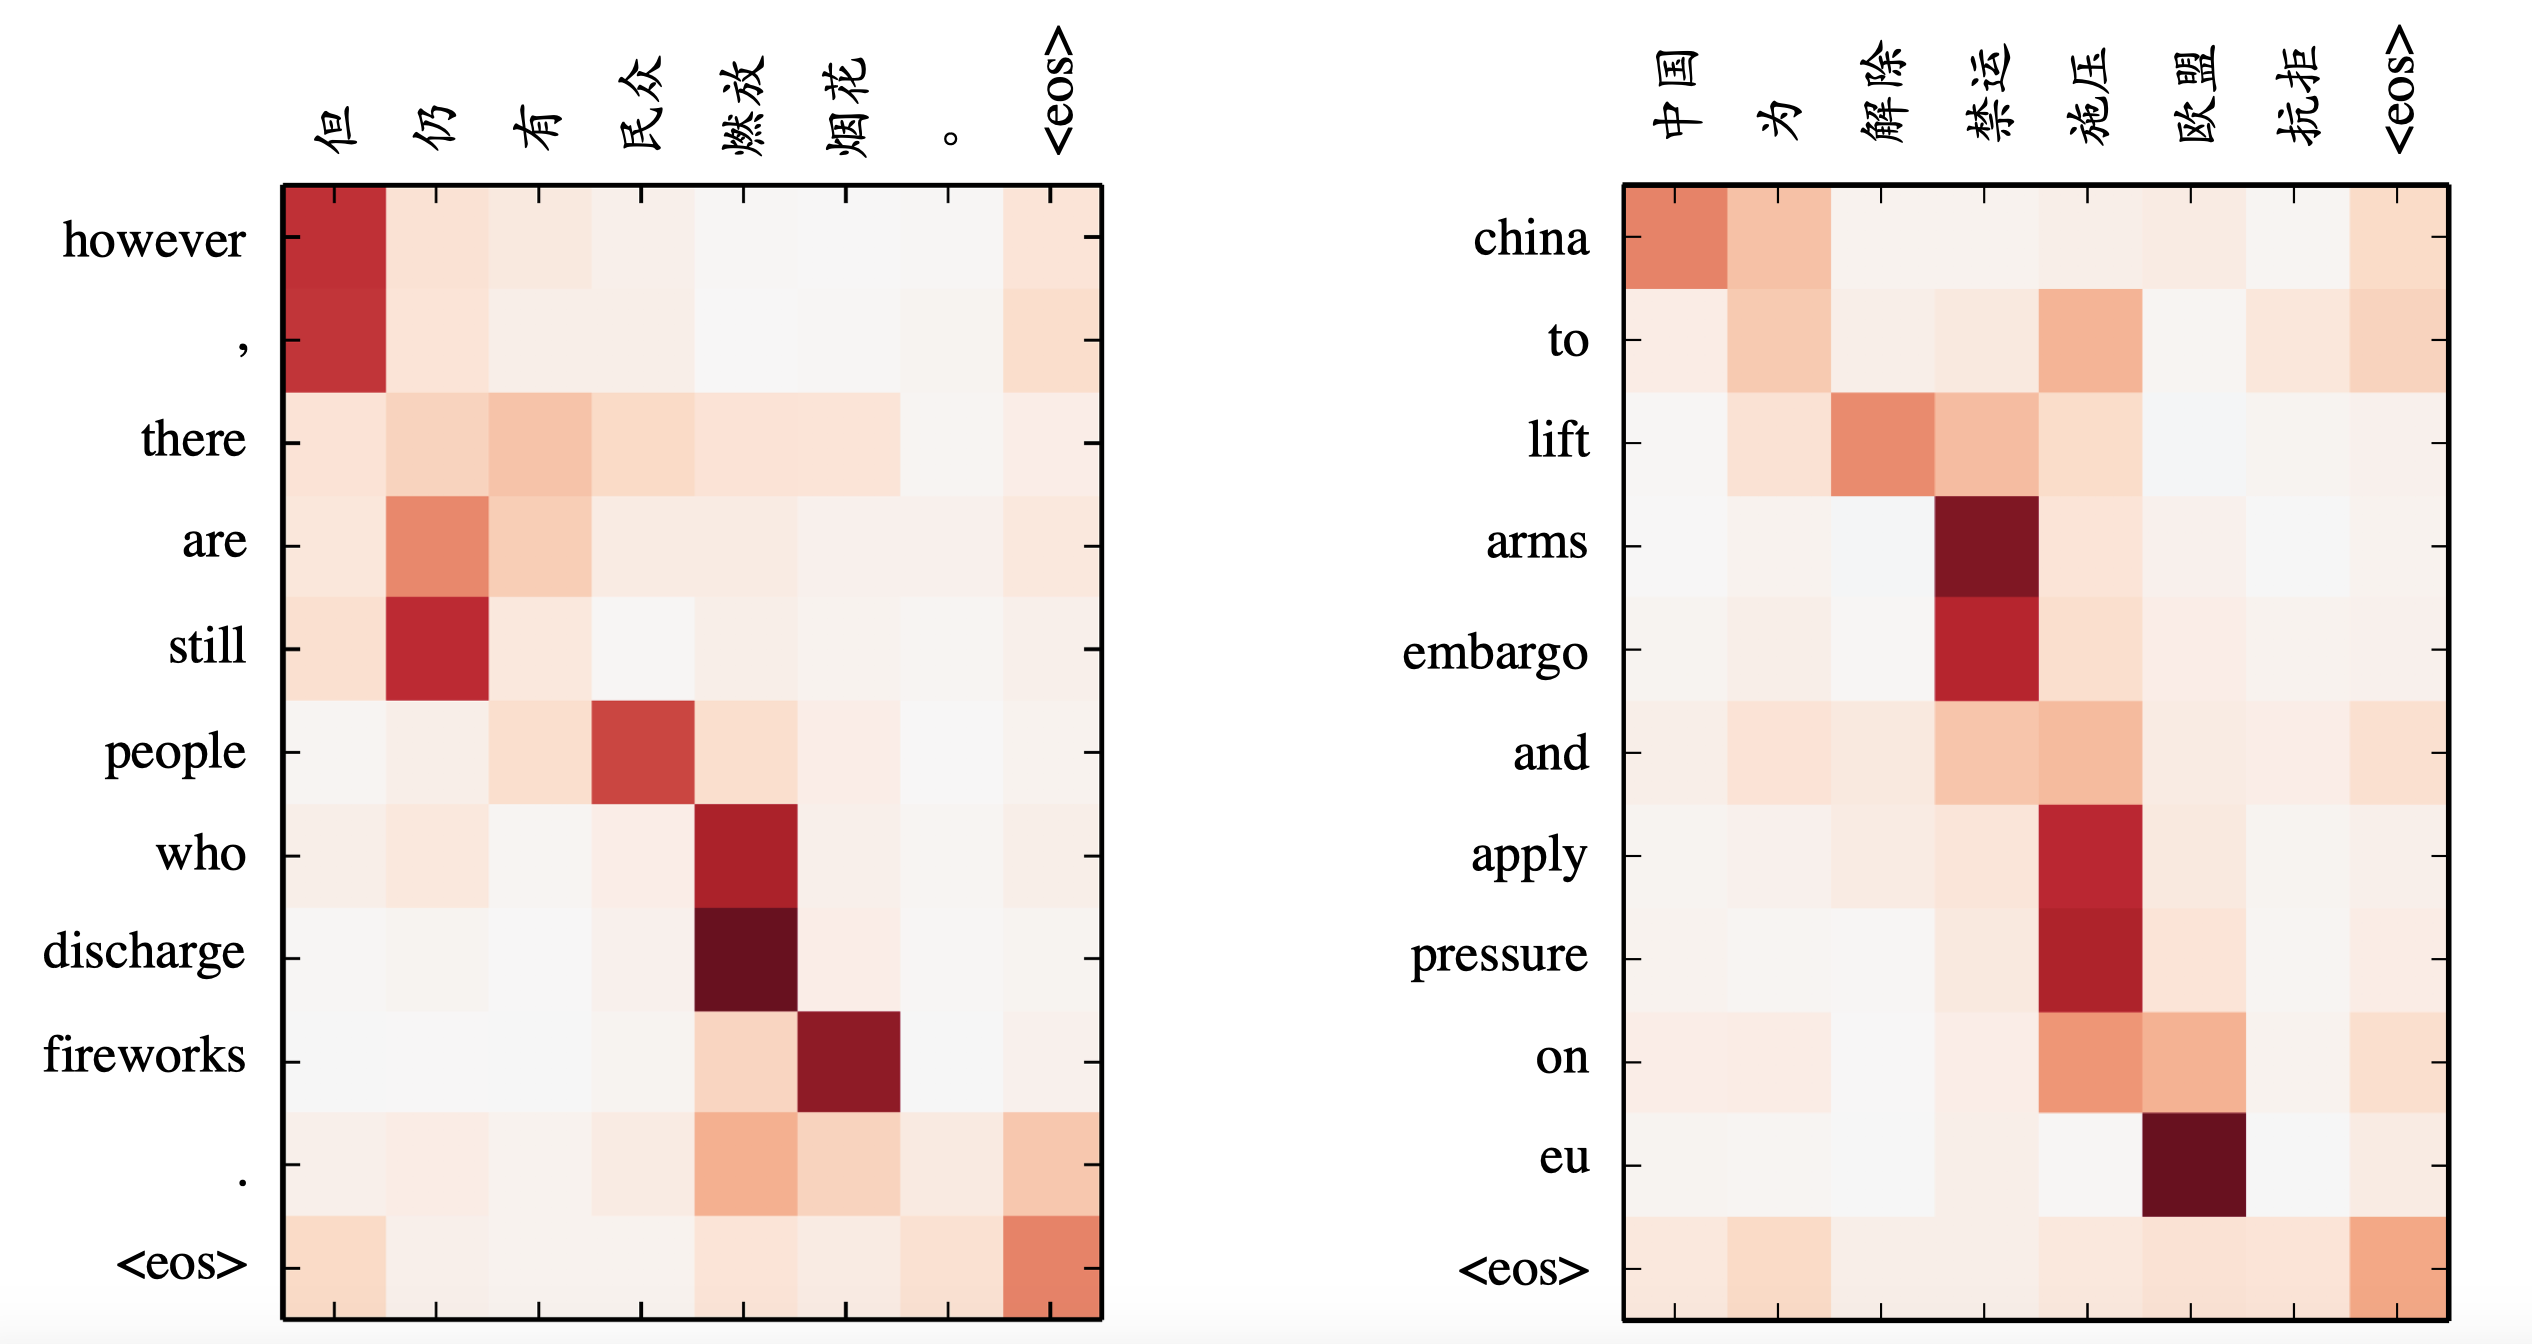
\includegraphics[width=1\textwidth]{fig/vis_transformer.pdf}
    \caption{Visualizing the relevance between source and target words.}
    \label{fig:visualization}
\end{figure}


\section{Installation}

\subsection{System Requirements}
THUMT supports Linux i686 and Mac OSX. The following third-party software and toolkits are required to install and use THUMT:
\begin{enumerate}
\item \verb|Python| v2.7.0 or higher;
\item \verb|TensorFlow| v1.6.0 or higher.
\end{enumerate}

\subsection{Installing THUMT}
The source code of THUMT is available at \href{https://github.com/thumt/THUMT}{https://github.com/thumt/THUMT}. Here is a brief guide on how to install THUMT.

\subsubsection{Step1: Downloading the Package}
Download the package using the following command:
\\
\begin{everbatim}
$ git clone https://github.com/thumt/THUMT.git
\end{everbatim}
\\
Entering the \verb|THUMT| folder, you may find two folders (\verb|thumt|, \verb|docs|) and three files (\verb|LICENSE|, \verb|README.md|, \verb|UserManual.pdf|):
\begin{enumerate}
\item \verb|thumt|: the source code;
\item \verb|docs|: LaTex files of the user manual;
\item \verb|LICENSE|: license statement;
\item \verb|README.md|: the readme formatted with Markdown;
\item \verb|UserManual.pdf|: this document.
\end{enumerate}

\subsubsection{Step 2: Modifying Environment Variables}
We highly recommend running THUMT on GPU servers. Suppose THUMT runs on NVIDIA GPUs with \href{https://developer.nvidia.com/cuda-toolkit}{the CUDA toolkit} v9.0 installed. Users need to set environment variables to enable the GPU support:
\\
\begin{everbatim}
$ export PATH=/usr/local/cuda/bin:$PATH
$ export LD_LIBRARY_PATH=/usr/local/cuda/lib64:$LD_LIBRARY_PATH
$ export PYTHONPATH=/PATH/TO/THUMT:$PYTHONPATH
\end{everbatim}
\\
To set these environment variable permanently for all future bash sessions, users can simply add the above three lines to the \verb|.bashrc| file in your \verb|$HOME| directory, where ``\verb|/PATH/TO/THUMT|'' is the path to the \verb|THUMT| folder.

\section{User Guide}

\subsection{Data Preparation}
\subsubsection{Obtaining the Datasets}
Running THUMT involves three types of datasets:

\begin{enumerate}
\item {\em Training set}: a set of parallel sentences used for training NMT models.
\item {\em Validation set}: a set of source sentences paired with single or multiple target translations used for model selection and hyper-parameter optimization.
\item {\em Test set}: a set of source sentences paired with single or multiple target translations used for evaluating translation performance on unseen texts.
\end{enumerate}

In this user manual, we take the preprocessed German-English dataset of the WMT 2017 news translation shared task as an example.\footnote{\href{http://data.statmt.org/wmt17/translation-task/preprocessed/de-en/}{http://data.statmt.org/wmt17/translation-task/preprocessed/de-en/}}  Download and unpack the two files \verb|corpus.tc.de.gz| and \verb|corpus.tc.en.gz|:
\\
\begin{everbatim}
$ gunzip corpus.tc.de.gz corpus.tc.en.gz
\end{everbatim}
\\
The resulting files \verb|corpus.tc.de| and \verb|corpus.tc.en| serve as the training set, which contains 5,852,458 pairs of sentences. Note that the German and English sentences are tokenized and truecased.

Unpack the file \verb|dev.tgz| using the following command:
\\
\begin{everbatim}
$ tar xvfz dev.tgz
\end{everbatim}
\\
In the \verb|dev| folder,  \verb|newstest2014.tc.de| and \verb|newstest2014.tc.en| serve as the validation set, which contains 3,003 pairs of sentences. The test set we use is \verb|newstest2015.tc.de| and \verb|newstest2015.tc.en|, which consists of 2,169 pairs of sentences. Note that both the validation and test sets use single references since there is only one gold-standard English translation for each German sentence.

\subsubsection{Running BPE}

For efficiency reasons, only a fraction of the full vocabulary can be used in neural machine translation systems. The most widely used  approach for addressing the open vocabulary problem is to use the Byte Pair Encoding (BPE) \citep{Sennrich:16}. We recommend using BPE for THUMT.

First, download the source code of BPE using the following command:
\\
\begin{everbatim}
$ git clone https://github.com/rsennrich/subword-nmt.git
\end{everbatim}
\\

To encode the training corpora using BPE, you need to generate BPE operations first. The following command will create a file named \verb|bpe32k|, which contains 32k BPE operations. It also outputs two dictionaries named \verb|vocab.de| and \verb|vocab.en|.
\\
\begin{everbatim}
$ python subword-nmt/learn_joint_bpe_and_vocab.py --input
corpus.tc.de corpus.tc.en -s 32000 -o bpe32k --write-vocabulary
vocab.de vocab.en
\end{everbatim}
\\
Then, the \verb|apply_bpe.py| script runs to encode the training set using the generated BPE operations and dictionaries.
\\
\begin{everbatim}
$ python subword-nmt/apply_bpe.py --vocabulary vocab.de
--vocabulary-threshold 50 -c bpe32k < corpus.tc.de >
corpus.tc.32k.de
$ python subword-nmt/apply_bpe.py --vocabulary vocab.en
--vocabulary-threshold 50 -c bpe32k < corpus.tc.en >
corpus.tc.32k.en
\end{everbatim}
\\

The validation set also needs to be processed using the \verb|apply_bpe.py| script.
\\
\begin{everbatim}
$ python subword-nmt/apply_bpe.py --vocabulary vocab.de
--vocabulary-threshold 50 -c bpe32k < newstest2014.tc.de >
newstest2014.tc.32k.de
$ python subword-nmt/apply_bpe.py --vocabulary vocab.en
--vocabulary-threshold 50 -c bpe32k < newstest2014.tc.en >
newstest2014.tc.32k.en
\end{everbatim}
\\
Finally, the source side of the test side is processed as well.
\\
\begin{everbatim}
$ python subword-nmt/apply_bpe.py --vocabulary vocab.de
--vocabulary-threshold 50 -c bpe32k < newstest2015.tc.de >
newstest2015.tc.32k.de
\end{everbatim}

\subsubsection{Shuffling Training Set}
The next step is to shuffle the training set, which proves to be helpful for improving the translation quality. Simply run the following command:
\\
\begin{everbatim}
$ python THUMT/thumt/scripts/shuffle_corpus.py --corpus
corpus.tc.32k.de corpus.tc.32k.en --suffix shuf
\end{everbatim}
\\
The resulting files \verb|corpus.tc.32k.de.shuf| and \verb|corpus.tc.32k.en.shuf| rearrange the sentence pairs randomly.

\subsubsection{Generating Vocabularies}
We need to generate vocabulary from the shuffled training set. This can be done by running the \verb|build_vocab.py| script:
\\
\begin{everbatim}
$ python THUMT/thumt/scripts/build_vocab.py corpus.tc.32k.de.shuf
vocab.32k.de
$ python THUMT/thumt/scripts/build_vocab.py corpus.tc.32k.en.shuf
vocab.32k.en
\end{everbatim}
\\
The resulting files \verb|vocab.32k.de.txt| and \verb|vocab.32k.en.txt| are final source and target vocabularies used for model training.

\subsection{Training}

\subsubsection{Transformer}
We recommend using the Transformer model that delivers the best translation performance among all the three models supported by THUMT.

The command for training a Transformer model is given by
\\
\begin{everbatim}
$ python THUMT/thumt/bin/trainer.py --input corpus.tc.32k.de.shuf
corpus.tc.32k.en.shuf --vocabulary vocab.32k.de.txt
vocab.32k.en.txt --model transformer --validation
newstest2014.tc.32k.de --references newstest2014.tc.32k.en
--parameters=batch_size=6250,device_list=[0],update_cycle=4,
train_steps=200000
\end{everbatim}
\\
Note that we set the \verb|batch_size| on each device (e.g. GPU) to 6,250 words instead of 6,250 sentences. By default, the batch size for the Transformer model is defined in terms of word number rather than sentence number in THUMT. We set \verb|update_cycle| to 4, which means the model parameters are updated every 4 batches. This effectively simulates the setting of ``\verb|batch_size|=25,000'' and requires less GPU memory.

``\verb|device_list=[0]|'' suggests that \verb|gpu0| is used to train the model. THUMT supports to train NMT models on multiple GPUs. If both \verb|gpu0| and \verb|gpu1| are available, simply set ``\verb|device_list=[0,1],update_cycle=2|''. You may use the \verb|nvidia-smi| command to find unused GPUs.

By setting ``\verb|train_steps=200000|'', the training process will terminate at iteration 200,000. During the training, the \verb|trainer.py| script creates a \verb|train| folder to store intermediate models called {\em checkpoints}, which will be evaluated on the validation set periodically. Only a small number of checkpoints that achieves highest BLEU scores on the validation set will be saved in the \verb|train/eval| folder. This folder will be used in decoding. Please refer to Appendix \ref{appendix:1} for more details about the parameters of the \verb|trainer.py| script.

\subsubsection{RNNsearch}

The command for training an RNNsearch model is given by
\\
\begin{everbatim}
$ python THUMT/thumt/bin/trainer.py --input corpus.tc.32k.de.shuf
corpus.tc.32k.en.shuf --vocabulary vocab.32k.de.txt
vocab.32k.en.txt --model rnnsearch --validation
newstest2014.tc.32k.de --references newstest2014.tc.32k.en
--parameters=batch_size=128,device_list=[0],train_steps=200000
\end{everbatim}
\\
Note that we set the \verb|batch_size| to 128 sentences instead of 128 words. By default, the batch size for the RNNsearch model is defined in terms of sentence number rather than word number in THUMT. The trained models are also saved in the \verb|train/eval| folder.

\subsubsection{Seq2Seq}

The command for training a Seq2Seq model is given by
\\
\begin{everbatim}
$ python THUMT/thumt/bin/trainer.py --input corpus.tc.32k.de.shuf
corpus.tc.32k.en.shuf --vocabulary vocab.32k.de.txt
vocab.32k.en.txt --model seq2seq --validation
newstest2014.tc.32k.de --references newstest2014.tc.32k.en
--parameters=batch_size=128,device_list=[0],train_steps=200000
\end{everbatim}
\\
Note that we set the \verb|batch_size| to 128 sentences instead of 128 words. By default, the batch size for the Seq2Seq model is  also defined in terms of sentence number rather than word number in THUMT. The trained models are saved in the \verb|train/eval| folder as well.

\subsection{Decoding}

The command for translating the test set using the trained Transformer model is given by
\\
\begin{everbatim}
$ python THUMT/thumt/bin/translator.py --models transformer
--input newstest2015.tc.32k.de --output newstest2015.trans
--vocabulary vocab.32k.de.txt vocab.32k.en.txt 
--checkpoints train/eval --parameters=device_list=[0]
\end{everbatim}
\\
The commands for using RNNsearch and Seq2Seq models are similar except for the \verb|--models| argument. The translation file output by the \verb|translator.py| is \verb|newstest2015.trans|, which needs to be restored to the normal tokenization using the following command:
\\
\begin{everbatim}
$ sed -r 's/(@@ )|(@@ ?$)//g' < newstest2015.trans >
newstest2015.trans.norm
\end{everbatim}
\\
Finally, BLEU scores \citep{Papineni:02} can be calculated using the \verb|multi-bleu.perl|\footnote{\href{https://github.com/moses-smt/mosesdecoder/blob/master/scripts/generic/multi-bleu.perl}{https://github.com/moses-smt/mosesdecoder/blob/master/scripts/generic/multi-bleu.perl}}:
\\
\begin{everbatim}
$ multi-bleu.perl -lc newstest2015.tc.en
< newstest2015.trans.norm > evalResult
\end{everbatim}
\\
The resulting \verb|evalResult| stores the calculated BLEU score.

\subsection{Visualizing}

The command for computing the relevances between source sentences and their translation using a trained Transformer model is given by
\\
\begin{everbatim}
$ python THUMT/thumt/bin/get_relevance.py --model transformer 
--input newstest2015.tc.32k.de --output newstest2015.trans
--vocabulary vocab.32k.de.txt vocab.32k.en.txt 
--checkpoints train/eval --relevances lrp_newstest2015
--parameters=device_list=[0]
\end{everbatim}
\\
The command for using RNNsearch model is similar except for the \verb|--models| argument. The relevance matrix of each sentence pair is stored in an individual file in the directory \verb|lrp_newstest2015|. To visualize the relevance between the n-th sentence and its translation, use the following command:
\\
\begin{everbatim}
$ python THUMT/thumt/scripts/visualize.py lrp_newstest2015/n
\end{everbatim}
\\

\section{FAQ}

\subsection{Does THUMT support multiple GPUs?}
Yes. THUMT supports to train NMT models on multiple GPUs. You may use the \verb|nvidia-smi| command to find unused GPUs. If both \verb|gpu0| and \verb|gpu1| are available, simply set ``\verb|device_list=[0,1]|'' when running the \verb|trainer.py| script.

\subsection{Does THUMT support model averaging?}

Yes. THUMT uses the \verb|checkpoint_averaging.py| script to average checkpoints generated during training to generate a better model. The script is located in the \verb|THUMT/thumt/scripts| folder. Simply run the following command:
\\
\begin{everbatim}
$ python THUMT/thumt/scripts/checkpoint_averaging.py --path train
--checkpoints 5 --output averaged
\end{everbatim}
\\
By default, the \verb|train| folder saves the last 20 checkpoints. The above command averages the last 5 checkpoints and saves the averaged model in the \verb|averaged| folder. You may change the number of checkpoints by modifying the \verb|--checkpoints| argument.

\subsection{Does THUMT support model ensemble?}

Yes. Suppose THUMT runs four times on the same training data. Due to random initialization, the four trained models are different. The following command can be used to ensemble the four models located in four separated folders (e.g., \verb|run1|, \verb|run2|, \verb|run3|, and \verb|run4|):
\\
\begin{everbatim}
$ python THUMT/thumt/bin/translator.py --models transformer
--input newstest2015.tc.32k.de --output newstest2015.trans
--vocabulary vocab.32k.de vocab.32k.en
--checkpoints run1/train run2/train run3/train run4/train
--parameters=device_list=[0]
\end{everbatim}

\subsection{How to save disk space during training?}

During training, latest checkpoints are stored in the \verb|train| folder. The number of checkpoints is specified by the \verb|keep_checkpoint_max| parameter in the \verb|trainer.py| script. Its default value is 20.

Checkpoints with top BLEU scores on the validation set are stored in the \verb|train/eval| folder. The number is specified by the \verb|keep_top_checkpoint_max| parameter in the \verb|trainer.py| script. Its default value is 5.

The size of a checkpoint is usually about 1GB. As a result, by default, the \verb|train| folder that stores intermediate files often takes up 30GB of disk space. To save disk space, simply set the two parameters to smaller values. For example, we can set \verb|keep_checkpoint_max| to 5 to keep only 5 checkpoints in the \verb|train| folder and \verb|keep_top_checkpoint_max| to 1 to keep only 1 checkpoint in the \verb|train/eval| folder. Note that \verb|keep_checkpoint_max| also determines the maximum number of checkpoints that can be used for model averaging.

An example command is shown below:
\\
\begin{everbatim}
$python THUMT/thumt/bin/trainer.py --input corpus.tc.32k.de.shuf
corpus.tc.32k.en.shuf --vocabulary vocab.32k.de.txt
vocab.32k.en.txt --model transformer --validation
newstest2014.tc.32k.de --references newstest2014.tc.32k.en
--parameters=batch_size=6250,device_list=[0],train_steps=200000,
keep_checkpoint_max=5,keep_top_checkpoint_max=1
\end{everbatim}

\subsection{How to display the BLEU scores on the validation set?}
It often takes several days to run THUMT on large training data. To prevent the command from being aborted if you log out or exit the shell, we recommend prefixing a command with \verb|nohup| and appending a ``\verb|&|'' symbol at the end of the command. For example,
\\
\begin{everbatim}
$ nohup python THUMT/thumt/bin/trainer.py --input
corpus.tc.32k.de.shuf corpus.tc.32k.en.shuf --vocabulary
vocab.32k.de.txt vocab.32k.en.txt --model transformer
--validation newstest2014.tc.32k.de --references
newstest2014.tc.32k.en --parameters=batch_size=6250,
device_list=[0],train_steps=200000,eval_step=5000 &
\end{everbatim}
\\
Output that would normally go to the terminal goes to a file called \verb|nohup.out|. Since the parameter \verb|eval_step| is set to 5,000, the intermediate model will be validated for every 5,000 steps. Here is an example output for validation:
\\
\begin{everbatim}
INFO:tensorflow:Validating model at step 5000
INFO:tensorflow:Restoring parameters from train/model.ckpt-5000
INFO:tensorflow:BLEU at step 5000: 0.283899
INFO:tensorflow:Copying train/model.ckpt-5000 to train/eval/
model.ckpt-5000
INFO:tensorflow:Best score at step 5000: 0.283899
\end{everbatim}
\\

Therefore, you may run the following command to obtain all BLEU scores on the validation set:
\\
\begin{everbatim}
$ grep 'BLEU at step' nohup.out
INFO:tensorflow:BLEU at step 5000: 0.215739
INFO:tensorflow:BLEU at step 10000: 0.274530
INFO:tensorflow:BLEU at step 15000: 0.295066
INFO:tensorflow:BLEU at step 20000: 0.310839
INFO:tensorflow:BLEU at step 25000: 0.314701
INFO:tensorflow:BLEU at step 30000: 0.324403
INFO:tensorflow:BLEU at step 35000: 0.326532
INFO:tensorflow:BLEU at step 40000: 0.327123
INFO:tensorflow:BLEU at step 45000: 0.331918
INFO:tensorflow:BLEU at step 50000: 0.335435
INFO:tensorflow:BLEU at step 55000: 0.333007
INFO:tensorflow:BLEU at step 60000: 0.337739
INFO:tensorflow:BLEU at step 65000: 0.342414
INFO:tensorflow:BLEU at step 70000: 0.343452
INFO:tensorflow:BLEU at step 75000: 0.344703
INFO:tensorflow:BLEU at step 80000: 0.342933
INFO:tensorflow:BLEU at step 85000: 0.345208
INFO:tensorflow:BLEU at step 90000: 0.345368
INFO:tensorflow:BLEU at step 95000: 0.345791
INFO:tensorflow:BLEU at step 100000: 0.348987
INFO:tensorflow:BLEU at step 105000: 0.349707
INFO:tensorflow:BLEU at step 110000: 0.346962
INFO:tensorflow:BLEU at step 115000: 0.348421
INFO:tensorflow:BLEU at step 120000: 0.349368
INFO:tensorflow:BLEU at step 125000: 0.347384
INFO:tensorflow:BLEU at step 130000: 0.351331
INFO:tensorflow:BLEU at step 135000: 0.350806
INFO:tensorflow:BLEU at step 140000: 0.351425
INFO:tensorflow:BLEU at step 145000: 0.350630
INFO:tensorflow:BLEU at step 150000: 0.349003
INFO:tensorflow:BLEU at step 155000: 0.353210
INFO:tensorflow:BLEU at step 160000: 0.352494
INFO:tensorflow:BLEU at step 165000: 0.353489
INFO:tensorflow:BLEU at step 170000: 0.351439
INFO:tensorflow:BLEU at step 175000: 0.352664
INFO:tensorflow:BLEU at step 180000: 0.352319
INFO:tensorflow:BLEU at step 185000: 0.353467
INFO:tensorflow:BLEU at step 190000: 0.354170
INFO:tensorflow:BLEU at step 195000: 0.352935
INFO:tensorflow:BLEU at step 200000: 0.353187
\end{everbatim}
\\

\appendix

\section{Parameters of The trainer.py Script} \label{appendix:1}
The parameters of the \verb|trainer.py| scripts is specified by a string containing comma-separated \verb|name=value| pairs. Here, we list important parameters in detail.

\subsection{General Parameters}
\begin{enumerate}
\item \verb|num_threads|: the number of threads used in data processing. The default value is 6.
\item \verb|buffer_size|: the buffer size used in data processing. The default value is 10,000.
\item \verb|batch_size|: the batch size used in the training stage. The default value is 4096.
\item \verb|constant_batch_size|: a boolean value that specifies whether the number of sentences is treated as \verb|batch_size|. The default value is \verb|true|. If it is set to \verb|true|, \verb|batch_size| is defined as the number of sentences. This usually happens for training Seq2Seq and RNNsearch models. If it is set to \verb|false|, \verb|batch_size| is defined as the number of tokens, which is more appropriate for training the Transformer model.
\item \verb|max_length|: the maximum length of a sentence in the training set. The default value is 256.
\item \verb|train_steps|: the total number of steps in the training stage. The default value is 100,000.
\item \verb|update_cycle|:  the number of iterations for updating model parameters. The default value is 1. If you have only 1 GPU and want to obtain the same translation performance with using 4 GPUs, simply set this parameter to 4. Note that the training time will also be prolonged.
\item \verb|save_checkpoint_steps|: the number of steps for saving a checkpoint periodically.  The default value is 1,000.
%\item \verb|save_checkpoint_secs|: the number of seconds for saving a checkpoint periodically. The default value is 0.
\item \verb|initializer|: choose how to initialize model parameters. Possible values are \verb|uniform|, \verb|normal|, \verb|uniform_unit_scaling|, and \verb|normal_unit_scaling|. The default value is \verb|uniform_unit_scaling|.
\item \verb|initializer_gain|: set the parameter of the initializer. The default value is 1.0.
\item \verb|learning_rate|: set the learning rate. The default value is 1.0.
\item \verb|learning_rate_decay|: set learning rate decay function. Possible values are \verb|linear_warmup_rsqrt_decay|, \verb|piecewise_constant|, and \verb|none|. The default value is \verb|linear_warmup_rsqrt_decay|.
\item \verb|learning_rate_boundaries|: learning rate boundaries. The default value is $[0]$.
\item \verb|learning_rate_values|: learning rate values. The default value is $[0.0]$.
\item \verb|keep_checkpoint_max|: the maximum number of checkpoints to keep during training. The default value is 20.
\item \verb|keep_top_checkpoint_max|: the maximum number of top performed checkpoints to keep during training. The default value is 5.
\item \verb|eval_steps|: the number of steps for evaluating the intermediate model periodically on the validation set. The default value is 2,000.
%\item \verb|eval_secs|: the number of seconds for evaluating the intermediate model periodically on the validation set. The default value is 0.
\item \verb|eval_batch_size|: the batch size for evaluating the intermediate model periodically on the validation set. The default value is 32.
\item \verb|beam_size|: beam size for beam search in decoding. The default value is 4.
\item \verb|decode_alpha|: the length penalty term in the beam search \citep{Wu:16}. The default value is 0.6.
\item \verb|decode_length|: the maximum length ratio of a translation. The default value is 50.
\item \verb|device_list|: the list of GPUs to be used in training. Use the \verb|nvidia-smi| command to find unused GPUs. If the unused GPUs are \verb|gpu0| and \verb|gpu1|, set this parameter as \verb|device_list=[0,1]|.
\item \verb|only_save_trainable|: choose which variables to keep. If it is set to \verb|true|, then only trainable variables will be saved in checkpoint. Otherwise, all variables (including variables created by optimizers) will be saved. Set this value to \verb|true| if you want to save disk space.
\end{enumerate}

\subsection{Parameters for Seq2Seq}

\begin{enumerate}
\item \verb|rnn_cell|: the recurrent unit. Possible values are \verb|LSTMCell| and \verb|GRUCell|. The default value is \verb|LSTMCell|.
\item \verb|embedding_size|: word embedding size for source and target languages. The default value is 1,000.
\item \verb|hidden_size|: the size of hidden layers. The default value is 1,000.
\item \verb|num_hidden_layers|: the number of hidden layers. the default value is 4.
\item \verb|dropout|: dropout rate. The default value is 0.2.
\item \verb|label_smoothing|: the value of label smoothing. The default value is 0.1.
\item \verb|reverse_source|: a boolean value that specifies whether the input sentence is reversed \citep{Sutskever:14}. The default value is \verb|true|.
\item \verb|use_residual|: a boolean value that specifies whether residual connections are used for multi-layered RNNs. The default value is \verb|true|.
\end{enumerate}

\subsection{Parameters for RNNsearch}

\begin{enumerate}
\item \verb|rnn_cell|: the recurrent unit. Currently, only GRU is supported. The default value is \verb|LegacyGRUCell|.
\item \verb|embedding_size|: word embedding size for source and target languages. The default value is 620.
\item \verb|hidden_size|: the size of hidden layers. The default value is 1,000.
\item \verb|maxnum|: the hidden units of maxout layer. The default value is 2.
\item \verb|dropout|: dropout rate. The default value is 0.2.
\item \verb|label_smoothing|: the value of label smoothing. The default value is 0.1.
\end{enumerate}

\subsection{Parameters for Transformer}
\begin{enumerate}
\item \verb|hidden_size|: the embedding size and hidden size of the network. The default value is 512.
\item \verb|filter_size|: the hidden size of the feed-forward layer. The default value is 2,048.
\item \verb|num_encoder_layers|: the number of encoder layers. The default value is 6.
\item \verb|num_decoder_layers|: the number of decoder layers. The default value is 6.
\item \verb|num_heads|: the number of attention heads used in the multi-head attention mechanism. The default value is 8.
\item \verb|shared_embedding_and_softmax_weights|: a boolean value that specifies whether to share the embedding and softmax weights. The default value is \verb|false|.
\item \verb|shared_source_target_embedding|: a boolean value that specifies whether to share the source and target embeddings. The default value is \verb|false|.
\item \verb|residual_dropout|: the dropout rate used in residual connection. The default value is 0.1.
\item \verb|attention_dropout|: the dropout rate used in attention mechanism. The default value is 0.0.
\item\verb|relu_dropout|: the dropout rate used in feed forward layer. The default value is 0.0.
\item \verb|label_smoothing|: the value of label smoothing. The default value is 0.1.
\end{enumerate}

\bibliographystyle{apalike}
\bibliography{thumt}

\end{document}
